\chapter{مروری بر کارهای پیشین}

\section{مقدمه}
در این فصل، به مرور کارهای گذشته می پردازیم.
مدل سیستم مقالات مختلف را معرفی کرده و مورد بررسی قرار می دهیم و نتایج عددی آن را نیز با یکدیگر مقایسه می نماییم.
\section{برش دینامیکی شبکه در ساختار رادیویی ابری متجانس}
در مقاله ی \cite{lee2018dynamic}
برش شبکه به صورت دینامیکی در بخش رادیویی مورد بررسی قرار گرفته شده است.
چارچوب طرح برش شبکه شامل یک سطح بالاتر، که مدیریت کنترل پذیرش، تشکل و تخصیص منابع باند پایه و یک سطح پایین تر، که تخصیص منابع رادیو در میان کاربران می باشد.
\subsection{مدل سیستم}
در این مدل فرض می کنیم که هر سرویس دارای شبکه اصلی خود (یا قطعه اصلی شبکه) است که به H-CRAN متصل می شود.
سلول بزرگ RRH (M-RRH) و سلولهای کوچک RRHs (S-RRHs) به ترتیب از طریق پیوندهای پشتی و fronthaul به یک استخر ابر
BBU  متصل می شوند.
همچنین ، تقسیم C/U در مدل سیستم فرض می شود، که به موجب آن صفحات کنترل و داده از هم جدا می شوند به گونه ای که صفحات کنترل توسط M-RRH در شبکه مدیریت می شود.
ما مشخصات LTE را دنبال می کنیم که در آن پهنای باند کانال به بلوک های منابع فیزیکی (PRBs) تقسیم می شود، هرکدام واحد منبع هستند که 180 کیلوهرتز را در دامنه فرکانس و 0.5 میلی ثانیه در دامنه زمان اشغال می کنند.
در LTE ، حداقل دو PRB (در حوزه زمان) می توانند به یک UE اختصاص دهند زیرا تخصیص منابع در هر بازه زمانی انتقال (TTI) از
$1ms$
 انجام می شود.
 در اینجا
$N$
سرویس، $U$ کاربر و $K$  منبع فیزیکی داریم. همچنین $S$ تا RRH داریم که RRH شماره ی $0$ مربوط به M-RRH  و بقیه ی RRH ها S-RRH می باشند.
$a_u$
متغیر باینری می باشد که نشان می دهد که کاربر $u$ ام در شبکه پذیرفته شده است یا نه.
$b_{su}$
 متغیر باینری می باشد که نشان می دهد که کاربر $u$ ام به $s$ امین RRH متصل است یا نه.
$w_{ksu}$
 متغیر باینری می باشد که نشان می دهد که کاربر $u$ ام به $s$ امین RRH متصل است و به این کاربر منبع فیزیکی $k$ ام داده شده است یا خیر.
 همچنین توان 
 کاربر $u$ ام که به $s$ امین RRH متصل است و به این کاربر منبع فیزیکی $k$ ام داده شده، $p_{ksu}$ می باشد.
 علاوه براین، ظرفیت محاسباتی BBU مجازی مورد نیاز برای کاربر $u$، 
 $c_{vB,u}$
  می باشد.
   همچنین فرض می کنیم که میزان منابع محاسباتی استخر BBU با ظرفیت داده کاربر به
   $C_{cBUP}$ 
   محدود شده است.
   اولویت کاربران را با 
   $\omega_u \in [0,1]$
   نشان می دهیم.
   اولویت سرویس ها را با 
   $v_n \in [0,1]$
   نشان می دهیم
   که 
   $\sum_n v_n =1$ 
   می باشد.
   در مدل سازی کانال، نسبت سیگنال به تداخل به علاوه نویز (SINR) که توسط کاربر u در RRH s در PRB
   k
     تجربه می شود ، بدین صورت مدل سازی شده است.
 \begin{equation}
 \rho_{sku} = \frac{p_{sku}g_{sku}}{P_{AWGN}+\sum_{i\in S/\{s\}}\sum_{j\in U/\{u\}}a_j b_{ij}w_{ijk}p_{ijk}g_{ijk}}.
 \end{equation}
 و داریم 
 \begin{equation}
 r_{sku} = B\log_2{(1+\rho_{sku})}.
 \end{equation}
 همچنین برای محدود کردن تداخل و استفاده از RRH ها و PRB ها حد بالای $I_{max,sku}$ تعریف می شود.
 به همین صورت برای توان مصرفی RRH  ها نیز حد بالای 
 $P_{max}$
تعریف می گردد.
هریک از S-RRH ها از طریق لینک 
fronthaul
 با ظرفیت
 $C_{fh}$
  به استخر BBU 
  وصل می شوند.
  M-RRH
   از طریق لینک
   backhaul
    با ظرفیت 
    $C_{bh}$ 
     به استخر BBU 
  وصل می شوند.
  مساله ی برش شبکه در بخش رادیویی در ادامه بیان می شود.
%\begin{equation}
%\begin{aligned}
%\max\limits_{a_u,b_{su},w_{sku},p_{sku},c_{vB,u}}   \quad &  \sum_{s\in S} \sum_{k\in K} \sum_{u\in U}
%v_n \omega_u a_u b_{su} w_{sku} r_{sku} \\
%\text{\lr{subject to}} \quad  & a_u\sum_{s\in S} \sum_{k\in K}  b_{su} w_{sku} r_{sku} \geq a_u R_{min,u} , \forall u,   \\
%& a_u\sum_{s\in S} \sum_{k\in K}  b_{su} w_{sku} r_{sku} \leq a_u c_{vB,u}  , \forall u,   \\
%& a_u\sum_{s\in S} \sum_{k\in K}  b_{su} w_{sku} r_{sku} \leq a_u R_{max,u}  , \forall u,   \\
%& \sum_{s\in S} \sum_{k\in K} a_u b_{su} w_{sku} r_{sku} \leq P_{max,s}  , \forall s,   \\
%& \sum_{s\in S} \sum_{k\in K} a_u b_{su} w_{sku} r_{sku} \leq C_{xh,s}  , \forall s,   \\
%&\sum_{i\in S/\{s\}}\sum_{j\in U/\{u\}}a_j b_{ij}w_{ijk}p_{ijk}g_{ijk} \leq I_{max,sku}  , \forall s, \forall k, \forall u   \\
%& a_u R_{min,u} \leq a_u c_{vB,u} \leq a_u R_{max,u} , \forall u,   \\
%& \sum_{u \in U} a_u c_{vB,u} \leq C_{cBUP} \\
%& \sum_{s \in S} a_u b_{su} \leq 1 \\ 
%& \sum_{u \in U} a_u b_{su} w_{sku} \leq 1 \\ 
%&  a_u, b_{su}, w_{sku} \in \{0,1\}  \forall s, \forall k, \forall u   \\ 
%& p_{sku},c_{vB,u} \geq 0 \\
%\end{aligned}	
%\end{equation}
\begin{figure}[H]
  \centering
    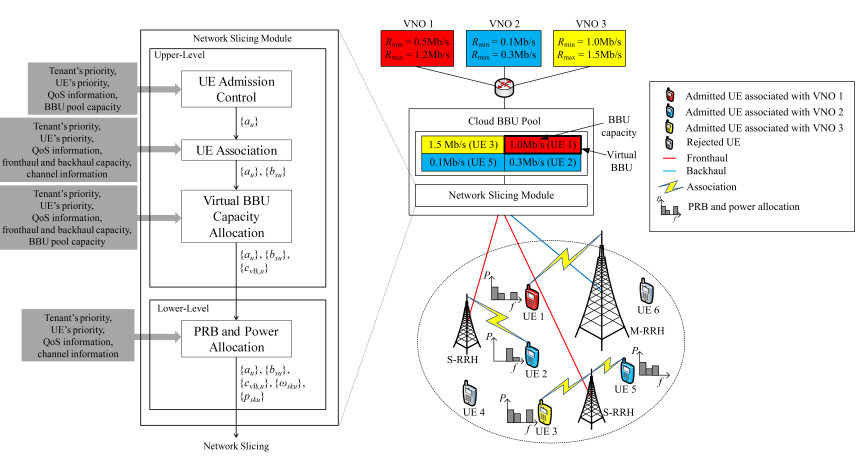
\includegraphics[scale = 0.7]{./fig/dynamicNS}
  \caption{روند برش شبکه\ \cite{lee2018dynamic}}
  \label{fig:dns}
\end{figure}
%برای حل این مسئله، می بایست مسئله را به بخش های کوچکتر تقسیم کرده و حل نماییم.
همانطور که در شکل \eqref{fig:dns} 
مشخص شده است ابتدا پذیرش کاربر مورد توجه قرار می گیرد و سپس کاربر به RRH متصل می شود و پس از آن ظرفیت BBU به آن تخصیص می دهد که تا این بخش از کار در سطح بالا قرار داریم و حال وارد الگوریتم سطح پایین تر می شویم که تخصیص توان و منبع فیزیکی می باشد.

\subsubsection{سطح بالا}
 \begin{enumerate}
 \item بررسی پذیرش کاربر
 
 در این بخش سعی می کنیم که تعداد کاربران پذیرفته شده در سیستم را افزایش دهیم.
 مسئله با فرض
  $c_{vB,u} \geq R_{min,u} $
   بدین صورت بیان می شود
  :
 \begin{equation}
 \begin{aligned}
 \max\limits_{b_{us}}   \quad &  \sum_{s\in S}\sum_{u\in U} W_{u} a_u  \\
\text{\lr{subject to}} \quad  & \sum_{u\in U} a_{u} R_{min,u}  \leq R_{cBUP} , \forall s,   \\
&  a_u \in \{0,1\}  \forall u   \\ 
 \end{aligned}	
 \end{equation}
 این بخش بوسیله ی روش دینامیکی حل می گردد.
 \item تخصیص به کاربران
 
 پس از اینکه تعدای از کاربران در شبکه پذیرفته شده و باقی از شبکه حذف شدند، حال به کاربران پذیرفته شده، RRH اختصاص داده می شود.
 ابتدا داریم:
  \begin{equation}
 \rho_{wb,su} = \frac{P_{max}\hat{g}_{su}}{P_{AWGN}+\sum_{i\in S/\{s\}}P_{max,i}\hat{g}_{iu}}.
 \end{equation}
 حال صورت مسئله بدین صورت است که با روش حریصانه حل می شود.
  \begin{equation}
 \begin{aligned}
 \max\limits_{b_{su}}   \quad &  \sum_{u\in U}\sum_{s\in S} W_{u} {b_{su}} \rho_{wb,su} \\
\text{\lr{subject to}} \quad  & \sum_{u\in U} b_{su} R_{min,u}  \leq C_{xh,s} , \forall u,   \\
& \sum_{s \in S}  b_{su} = 1 \\ 
&  {b_{su}} \in \{0,1\}  \forall u  \forall s  \\ 
 \end{aligned}	
 \end{equation}
 \item تخصیص ظرفیت BBU
 
بعد از پذیرش کاربران و تخصیص RRH به آنها، در این بخش ظرفیت BBU به کاربران تخصیص داده می شود که صورت مسئله در ادامه نوشته می شود و با روش simplex حل می گردد.
   \begin{equation}
 \begin{aligned}
 \max\limits_{c_{v,BU}}   \quad &  \sum_{u\in U} W_{u} {c_{v,BU}} \\
\text{\lr{subject to}} \quad  & \sum_{u\in U_{RRH}}c_{v,BU}  \leq C_{xh,s} , \forall u,   \\
&  R_{min,u} \leq  c_{vB,u} \leq  R_{max,u} , \forall u,   \\
& \sum_{s \in S}  c_{vB,u} \leq C_{cBUP} \\ 
&  c_{vB,u} \geq 0 , \forall u   \\
 \end{aligned}	
 \end{equation}
 \end{enumerate}
 \subsubsection{سطح پایین}
 پس از حل بخش قبلی در این بخش به تخصیص توان و بلوک های منابع فیزیکی می پردازیم.
 \begin{equation}
\begin{aligned}
\max\limits_{w_{sku},p_{sku}}   \quad &  \sum_{s\in S} \sum_{k\in K} \sum_{u\in U}
v_n \omega_u  w_{sku} r_{sku} \\
\text{\lr{subject to}} \quad  & \sum_{s\in S} \sum_{k\in K}  w_{sku} r_{sku} \geq R_{min,u} , \forall u,   \\
& \sum_{s\in S} \sum_{k\in K}   w_{sku} r_{sku} \leq  r_{vBBU,u}  , \forall u,   \\
& \sum_{s\in S} \sum_{k\in K} a_u b_{su} w_{sku} r_{sku} \leq P_{max,s}  , \forall s,   \\
&\sum_{i\in S/\{s\}}\sum_{j\in U/\{u\}}w_{ijk}p_{ijk}g_{ijk} \leq I_{max,sku}  , \forall s, \forall k, \forall u_{RRH}   \\
& \sum_{u \in U_{RRH}}  w_{sku} \leq 1 \\ 
&   w_{sku} \in \{0,1\}  \forall s, \forall k, \forall u   \\ 
& p_{sku} \geq 0 \\
\end{aligned}	
\end{equation}
که این مسئله نیز با روش لاگرانژ حل می گردد.
\section{برش شبکه به صورت زمان حقیقی }
در معماری برش شبکه، هر سرویس توسط برش خاصی پذیرفته می شود. همچنین هر سرویس دارای QoS ویژه ای است که باید به آن برسد. پارامترهای QoS شامل:
\begin{itemize}
\item تاخیر
\item نرخ ارسال داده
\item نرخ بسته های منتقل شده
\end{itemize}  
می باشد.
خدمات مختلف دارای یک یا چند مورد از این QoS هستند. روش های مبتنی بر هوش مصنوعی برای ارائه مزایای بالقوه برای رفع مشکلات و پیچیدگی های برش ، به تکنیک های امیدوار کننده تبدیل می شوند. ما می توانیم از روشهای مبتنی بر هوش مصنوعی برای پیش بینی دقیق ترافیک خاص سرویس استفاده کنیم.


فقط با چنین ترافیک خاص با سرویس دقیق پیش بینی شده ، برش RAN می تواند تخصیص منابع شبکه را برای تأمین خواسته های خدمات در آینده نزدیک تسهیل کند.
مطالعات اخیر نشان می دهد که روش های مبتنی بر هوش مصنوعی ، مانند شبکه عصبی عمیق (DNN) و حافظه کوتاه مدت بلند مدت (LSTM) ، قادر به پیش بینی دقیق بار ترافیکی خاص برای سرویس هستند.
روش های مبتنی بر هوش مصنوعی می توانند تخصیص منابع کارآمد در برش RAN را تسهیل کنند. یک فرایند تصمیم گیری در زمینه اختصاص منابع مبتنی بر هوش مصنوعی آنلاین ، پتانسیل دستیابی به یک پیچیدگی کم پس از یک روش آموزش آفلاین را دارد ، که به چالش پیچیدگی محاسباتی بالا در روش های بهینه سازی مبتنی بر مدل معمولی می پردازد.
  توجه داشته باشید که روش های سنتی RL مانند یادگیری Q از مشکل ابعاد زیاد رنج می برند که فقط برای مشکلات برش RAN در شبکه های در مقیاس کوچک مناسب هستند.

  روش های \lr{Deep RL } شامل شبکه های یادگیری عمیق در چارچوب RL می توانند به طور مؤثر مسائل پیچیدگی را در شبکه های در مقیاس بزرگ برطرف کنند
  \cite{aiNS}.
  \begin{figure}%[H]
  \centering  
    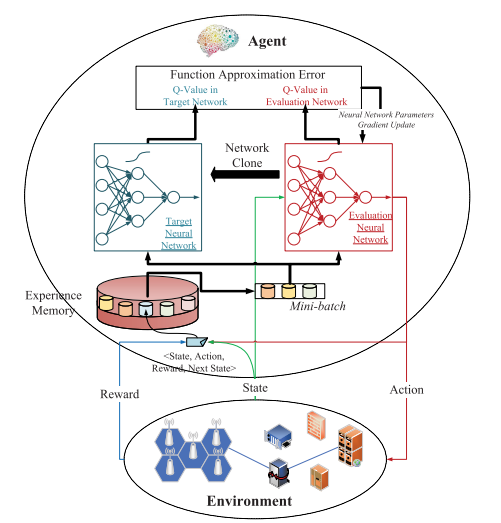
\includegraphics[scale = 0.7]{./fig/dlNS}
  \caption{ساختار یادگیری تقویت عمیق\cite{drl}}
  \label{fig:drl}
\end{figure}
\subsection{مدل سیستم}
در این بخش، یادگیری تقویت عمیق (DRL)\LTRfootnote{Deep Reinforcement Learning}، که به چگونگی تعامل با محیط با اقدامات جایگزین و تقویت اقدامات برای تولید پیامدهای پاداش دهنده تر می پردازد، فرض می شود که یک راه حل امیدوار کننده برای برش شبکه است\cite{drl}.
در این بخش هدف بیشینه کردن نرخ انتقال بر روی میزان پهنای باند مصرفی و همزمان بیشینه سازی درصد بسته های رسیده شده به کاربران می باشد.
 \begin{equation}
\begin{aligned}
\max\limits_{w_n}   \quad &  \alpha SE + \sum_{n\in N} \beta_n SSR_n  \\
\text{\lr{subject to}} \quad  & \sum_{u_n\in U_n} |Q_n| = d_n    \\
& \sum_{n\in W} w_n =1   \\
& x_{p_{u_n}} = 
\begin{cases}
      1 & r_{u_n} \geq \hat{r}_n, l_{p_{u_n}} \leq \hat{l}_n\\
      0 & \text{otherwise}
    \end{cases}  
\end{aligned}	
\end{equation} 
 که در اینجا، $\alpha$ وزن SE و $\beta_n$ وزن n امین SSR برای ایجاد برتری بین دو واحد SSR و SE می باشند.
 در اینجا SE
 نسبت نرخ انتقال به مجموع پهنای باند مصرفی می باشد
 \begin{equation}
 SE = \frac{\sum_{n\in N}\sum_{u_n\in U_n} r_{u_n}}{W}.
 \end{equation}
 در اینجا $w_n$ پهنای باند مصرفی n امین برش شبکه است و مجموع پهنای باند مصرفی با W نشان داده شده است.
 همچنین $r_{u_n}$ نرخ ارسالی در برش شبکه ی n می باشد.
 همچنین SSR درصد بسته های رسیده شده به کاربران می باشد که بدین صورت بیان می شود
 \begin{equation}
 SSR_n = \frac{\sum_{u_n\in U_n}\sum_{q_{u_n}\in Q_{u_n}}x_{q_{u_n}}}{\sum_{u_n\in U_n}|Q_n|}
 \end{equation}
 که در اینجا $|Q_n|$
 تعداد بسته های ارسالی به کاربر $u_n$ می باشد.
 همچنین $x_{q_{u_n}}$  اگر یک باشد بسته $q_{u_n}$ به کاربر $u_n$ رسیده است و اگر صفر باشد نرسیده است و در صورتی یک است که تاخیر $l_{q_{u_n}} \leq \hat{l}_n $
 باشد و نرخ 
 $r_{u_n} \geq \hat{r}_n $
 باشد\cite{gan1, gan2}.
 برای حل این سیستم مدل از ترکیب روش GAN
 با روش 
 Reinforcement learning
  استفاده می شود.
\section{برش شبکه با فرض سرویس های حساس به تاخیر و نرخ انتقال}
در این دسته مقالات، سرویس ها به دو بخش تقسیم می شوند در بخش اول سرویس هایی که  نسبت به تاخیر حساسند و دسته ی دوم سرویس هایی که نسبت به نرخ انتقال حساسند. همچنین در برخی مقالات هر دو ویژگی برای یک سرویس مد نظر می باشد.
در این مدل های سیستم، تاخیر با استفاده از M/M/1 در ساده ترین حالت یا برای نزدیک تر شدن به حالت حقیقی از M/D/1 نیز استفاده می شود. می توان در این مدل ها تاخیر را کمینه و نرخ انتقال را بیشینه کرده و یا 
برای کاربران نرخ را از حد مورد نیاز بیشتر و تاخیر را کمتر از حد مورد نیاز فرض کرد\cite{frdl,luong2018novel,luong2018novel1,guo2016exploiting}.
 \begin{figure}[H]
  \centering
    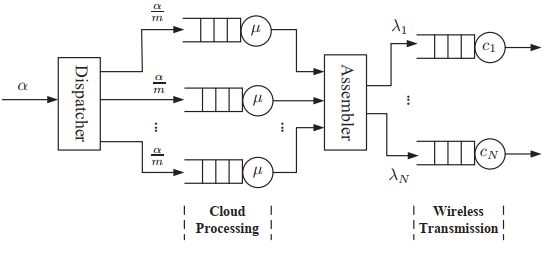
\includegraphics[scale = 0.7]{./fig/Delay}
  \caption{مدل پردازشی شبکه صف \cite{frdl}.}
  \label{fig:Delay}
\end{figure}
همانطور که در شکل \eqref{fig:Delay}، مشخص است، در این شبکه برای هر بخش تعدادی VNF قرار دارند که پردازش ها را انجام می دهند. در مسیر لینک پایین
بسته ها با نرخ $\alpha$ به صف های مختلف وارد شده و پس از پردازش با همدیگر ادغام شده و سپس بسته ی هر کاربر از طریق وایرلس منتقل می شوند.
در این پردازش ها، از روش M/M/1 استفاده شده است.

\section{جایگیری } 
 \section{ سیستمهای  \lr{MIMO C-RAN} در لینک فروسو }
در این قسمت، سیستمهای  \lr{MIMO C-RAN} در حالت فروسو مورد بررسی قرار می گیرد. در حالت فروسو،  واحد کنترل، پردازش اطلاعات پیام را با عملکرد کدگذاری کانال و پیش کد گذاری \LTRfootnote{precoding} مدیریت می نماید.
\subsection{مدل سیستم اول}
سیگنال پیش کدگذاری شده ی باند پایه در واحد کنترل، فشرده گشته و توسط لینک ارتباطی \lr{fronthaul} که دارای ظرفیت محدود است \cite{fc2}، به واحد رادیویی منتقل می گردد.
هر واحد رادیویی، از لینک \lr{fronthaul} سیگنالی را که دارای نویز کوانتیزاسیون است، دریافت می کند؛ سپس با اعمال \lr{pulse shaping}، سیگنال را به فرکانس بالاتر منتقل کرده و از طریق کانال بدون سیم به کاربران ارسال می نماید.
\begin{figure}[H]
  \centering
    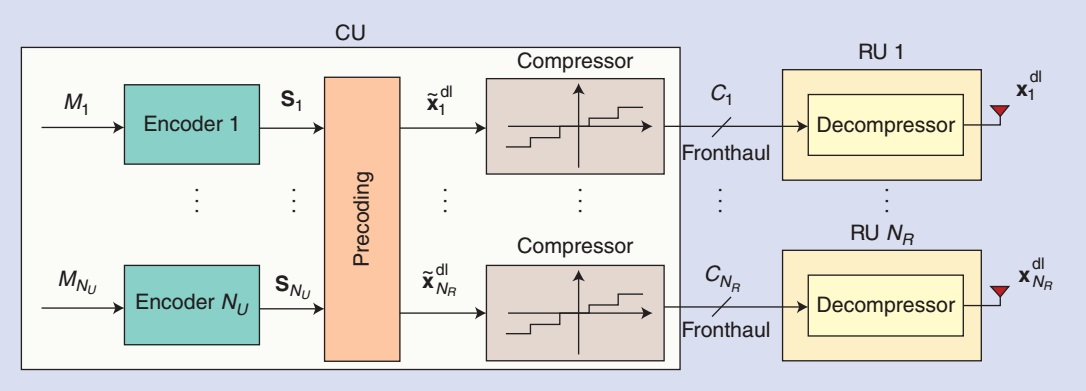
\includegraphics[width=\linewidth, height=6cm]{./fig/dl}
  \caption{مسیر انتقال پیام در لینک فروسو \cite{Fronthaul}.}
  \label{fig:dl}
\end{figure}
بلوک دیاگرام مدل سیستم اول
در شکل \ref{fig:dl} نشان شده است. 
در اینجا، $N_U$ کاربر قرار دارند که توسط $N_R$ واحد رادیویی سرویس دهی می شوند.


برای بدست آوردن سیگنال 
$\tilde{\boldsymbol{x}}^{dl}$ ،
واحد کنترل، سیگنال پیام را به صورت مجزا برای هر کاربر کدگذاری می کند.  با  اعمال این فرآیند،  سمبلهای $\boldsymbol{s}=[s_1;...;s_{N_U}]$  بدست می آید که $s_k$ نشان دهنده ی سمبل $k$ امین کاربر می باشد. 
سیگنال پیش کدگذاری شده ی
$\tilde{\boldsymbol{x}}^{dl} $
که توسط واحد کنترل تولید می گردد به این صورت بیان می شود:
\begin{equation}\label{wp}
 \tilde{\boldsymbol{x}}^{dl} = \boldsymbol{W}\boldsymbol{P}^{\frac{1}{2}} \boldsymbol{s},
\end{equation}
که 
 \begin{equation}
\tilde{\boldsymbol{x}}^{dl} = [\tilde{x}_{1}^{dl}; ... ; \tilde{x}_{N_R}^{dl}] 
 \end{equation}
 در رابطه ی  \eqref{wp}، $\boldsymbol{W}$، ماتریس پیش کدگذاری شده با ابعاد $N_R \times N_U$ می باشد و $\boldsymbol{W} = [\boldsymbol{w_1},..., \boldsymbol{w_{N_{U}}}]$ است. علاوه بر این، 
 $\boldsymbol{P}^{\frac{1}{2}} = diag(\sqrt{p_1},...,\sqrt{p_{N_U}})$ 
 ماتریس توان است.
حال سیگنال فشرده شده ی دریافتی توسط واحد رادیویی به صورت زیر بدست می آید:
\begin{equation}
\label{eq_pow1}
 {\boldsymbol{x}}^{dl} = \tilde{\boldsymbol{x}}^{dl} + \boldsymbol{Q},
\end{equation}
که در اینجا $\boldsymbol{Q} = \left[ q_1,\ldots,q_{N_R}\right]^T$، بردار نویز کوانتیزاسیون تولید شده به دلیل فشرده سازی بعد از پیش کدگذاری در واحد کنترل می باشد که دارای توزیع 
 $ \forall i  \quad  q_i\backsim \mathcal{N}(0,\sigma_{q_i^2}) $ 
 می باشد.
%%%%%%%%%%%%%%%%%%5
سیگنال دریافتی توسط $j$ امین کاربر به صورت $y_j$ نمایش داده می شود.
\begin{equation}
{y}_j = \boldsymbol{H}_j \boldsymbol{x}^{dl}+ z_j
\end{equation}
 $\boldsymbol{H}_j $
  بردار کانال کاربر $j$ام می باشد 
  که دارای ابعاد
 $1 \times N_R$ 
 است. همچنین
    $z_j$ نویز گوسی 
 $z_j \backsim \mathcal{N}(0,1) $ می باشد.
توان ارسالی از $i$ امین واحد رادیویی از رابطه ی زیر بدست می آید:
\begin{equation}\label{pr}
P_i (\boldsymbol{W},\sigma_q) = \frac{1}{T} E[{||{x_i}||}^2] = trace(\boldsymbol{w_i}\boldsymbol{P}^{\frac{1}{2}}(\boldsymbol{P}^H)^{ \frac{1}{2}}\boldsymbol{w_i}^H + \sigma_{q_i}^2 \boldsymbol{I})
\end{equation}
که در اینجا 
$T=1$
 می باشد.
همچنین 
$\sigma_{q_i}^2$
واریانس نویز کوانتیزاسیون است.
با توجه به رابطه ی \eqref{pr}
ظرفیت لینک \lr{fronthaul} از واحد کنترل به  $i$ امین واحد رادیویی 
از رابطه ی زیر بدست می آید:
\begin{equation}
C_i(\boldsymbol{W},\sigma_{q_i}) = \log det(\boldsymbol{w_i}\boldsymbol{P}^{\frac{1}{2}}(\boldsymbol{P}^H)^{ \frac{1}{2}}\boldsymbol{w_i}^H + \sigma_{q_i}^2 \boldsymbol{I}) - \log (\sigma_{q_i}^2)
\end{equation}
%%%%%%%%%%%%%%%%%%%%%%%%%%%%%5%%%%%%%%%
برای بدست آوردن نرخ قابل دسترس $j$ امین کاربر از فرمول زیر استفاده می گردد:

\begin{equation}
\boldsymbol{R}_j (\boldsymbol{W},\boldsymbol{\sigma_q})=I(s_j;y_j) 
\end{equation}
که در اینجا 
$I$
همان اطلاعات متقابل است.


 در این تحقیقات، مجموع نرخ های قابل دسترس براساس محدودیت ظرفیت لینک \lr{fronthaul} و محدودیت توان هر واحد رادیویی، بیشینه می گردد:
\begin{equation}
\begin{aligned}
\max\limits_{\boldsymbol{W},\boldsymbol{\sigma_q}}   \quad &   \sum_j R_j(\boldsymbol{W},\boldsymbol{\sigma_q})\\
\text{\lr{subject to}} \quad  & \bar{P}_i(\boldsymbol{W}, \sigma_q) \leq P_{max} \ \  \forall i \\
&C_i(\boldsymbol{W},\sigma_q)\leq C^{th}  \ \ \forall i \\
\end{aligned}
\end{equation}

 
%%%%%%%%%%%%%%%%%%%%%%%%%%%%%%%%%%%%%%%%%%%%%%%%%%%%%%%%%%%%%%%%%
در اینجا می خواهیم مجموع نرخ ها با محدودیت بیان شده را بیشینه کنیم. برای حل این مسائل از الگوریتم تکرار شونده و ضرایب لاگرانژ که در فصل بعدی ارائه می گردد، استفاده می شود \cite{ul_dl,ulSimeone, Fronthaul, precodSimeone, xia2018power}.

%%%%%%%%%%%%%%%%%%%%%%%%%%%%%%%%%%%%%%%%%%%%%%%%%%%%%%%%%%%
\subsection{مدل سیستم دوم}
در این بخش، مدل سیستم دومی را برای ساختار \lr{MIMO C-RAN} بررسی می کنیم. 


فرض بر این است که کاربران و \lr{RRH}ها، به 
 $S$
 تا خوشه تقسیم شده اند که $v$ امین خوشه،
 دارای $R_v$ تا \lr{RRH} است که ${D}_v$ تا کاربر را سرویس دهی می کنند.
همچنین  $r_{(s,n)}$
 نشان دهنده ی $n$ امین واحد رادیویی در $s$ امین خوشه می باشد  و به همین صورت $d_{(s,k)}$
 نشان دهنده ی $k$ امین کاربر در $s$ امین خوشه است.

 \begin{figure}[H]
  \centering
    \includegraphics[scale=1]{./fig/mimoCRAN}
  \caption{ساختار \lr{MIMO C-RAN} \cite{EEcluster}.}
  \label{fig:mimoC-RAN}
\end{figure}
در این قسمت، بردار سیگنال دریافتی کاربران در $s$ امین خوشه، به صورت زیر نوشته می شود:
\begin{equation} \label{sg}
\boldsymbol{y}_{\mathcal{D}_s} = \sum_{v=1}^S \boldsymbol{H}^H_{\mathcal{R}_v,\mathcal{D}_s}\boldsymbol{W}_{R_v, {D}_v}\boldsymbol{P}_{{D}_v}^\frac{1}{2}\boldsymbol{x}_{\mathcal{D}_v}+ \boldsymbol{z}_{\mathcal{D}_s},
\end{equation}
که در اینجا 
$\boldsymbol{x}_{ \mathcal{D}_v} = [x_{ d_{(v,1)}},..., x_{ d_{(v,D_v)}}]^T \in C^{ \mathcal{D}_v \times 1} $ 
بردار سمبل ارسالی واحد رادیویی از $t$ امین خوشه می باشد.

%%%%%%%%%%%%%%%%%%%%%%%%%%%%%%%%%%%%%%%%%%%%%%%%%%%%%%%
  $\boldsymbol{W}_{R_v, \boldsymbol{D}_v} = [\boldsymbol{w}_{ R_v,d_{(v,1)}},..., \boldsymbol{w}_{R_v, d_{(v,D_v)}}]^T \in C^{ R_v \times D_v} $ 
  ماتریس پیش کدگذاری اعمال شده در خوشه ی $v$ ام می باشد.
 علاوه بر این، $z_{D_s}$ نویز گوسی جمع شونده است که به صورت 
 $\boldsymbol{z_{\mathcal{D}_s}} \backsim \mathcal{N}(0,N_0\boldsymbol{I}_{{D}_s})$ 
و دارای توان $N_0$
می باشد.
همچنین $\boldsymbol{H}_{R_v,D_s}$ بردار کانال از واحدهای رادیویی دسته ی $R_v$ به کاربر دسته ی $D_s$ می باشد که این بردار را می توان به صورت زیر نوشت.
 $\boldsymbol{H}_{\mathcal{R}_v,\mathcal{D}_s}=\left[\boldsymbol{h}_{\mathcal{R}_v,d_{(s,1)}},\ldots,\boldsymbol{h}_{\mathcal{R}_v,d_{(s,\mathcal{D}_s)}}\right]^T  \in \mathbb{C}^{{R}_v\times {D}_s}$ 
 و همین طور
 بردار کانال از \lr{RRH} های خوشه ی  $v$ به $k$ امین کاربر در خوشه ی $s$ام  
 $\boldsymbol{h}_{\mathcal{R}_v,d_{(s,k)}}\in \mathbb{C}^{{R}_v}$
 به صورت زیر مدل می شود
 \begin{equation}\label{channel}
\boldsymbol{h}_{\mathcal{R}_v,d_{(s,k)}} = \boldsymbol{\beta}^\frac{1}{2}_{\mathcal{R}_v,d_{(s,k)}} \boldsymbol{g}_{\mathcal{R}_v,d_{(s,k)}},
\end{equation}
که  در اینجا $\boldsymbol{g}_{\mathcal{R}_v,d_{(s,k)}} \backsim \mathcal{N}(0,N_0\boldsymbol{I}_{\mathcal{D}_s})$ نشان دهنده ی بردار کانال محو شدگی سریع و مسطح برای کانال می باشد 
و $\boldsymbol{\beta}_{\mathcal{R}_v,d_{(s,k)}}=\text{\lr{diag}}(a_{r_{(v,1),d_{(s,k)}}},\ldots,a_{r_{(v,\mathcal{R}_v),d_{(s,k)}}})$
نشان دهنده ی محوشدگی  در مقیاس بزرگ می باشد. 
%%%%%%%%%%%%%%5
این مدل سیستم نیز شبیه به  مدل سیستم مسئله ی قبلی است با این تفاوت که در اینجا، فشرده سازی اعمال نمی گردد  $\boldsymbol{Q}_{\mathcal{R}_v} = \boldsymbol{0}$ و فرض این است که ظرفیت لینک  \lr{fronthaul} نامحدود است. 
به علاوه، در اینجا چندین خوشه باهم در نظر گرفته شده است و تداخل پیامها بین خوشه های متفاوت نیز محاسبه می شود.\newline
حال می خواهیم توان ارسالی از هر واحد رادیوی $i$ در خوشه ی $s$ به کاربران را محاسبه نمود.
\begin{equation}
\bar{p}_{r_{(s,i)}} = || \boldsymbol{w}_{r_{(s,i)},D_s}\boldsymbol{P}_{{D}_s}^\frac{1}{2}  ||^2
\end{equation} 
که در اینجا
$\boldsymbol{w}_{r_{(s,i)},D_s}$
سطر $i$ ام ماتریس $\boldsymbol{W}_{R_s, {D}_s}$
است.\newline
در حالت کلی برای بدست آوردن بردار کانال، در لینک فراسو با ارسال پایلوت، بردار کانال بدست می آید که در اینجا فرض می شود که با اندکی خطا همراه است و به این صورت بیام می گردد.
\begin{equation*}
\hat{\boldsymbol{h}}_{\mathcal{R}_v,d_{(s,k)}} = \boldsymbol{h}_{\mathcal{R}_v,d_{(s,k)}} + \Delta \boldsymbol{h}_{\mathcal{R}_v,d_{(s,k)}},
\end{equation*}

$\Delta \boldsymbol{h}_{\mathcal{R}_v,d_{(s,k)}}$
نشان دهنده ی بردار خطای تخمین زده شده است که دارای توزیع گوسی به صورت
$$\Delta \boldsymbol{h}_{\mathcal{R}_v,d_{(s,k)}}\backsim \mathcal{N}(0,\boldsymbol{\phi}_{\mathcal{R}_v,d_{(s,k)}}^2),$$
است که  داریم 
$$\boldsymbol{\phi}_{\mathcal{R}_v,d_{(s,k)}} = \text{\lr{diag}}(\phi_{r_{(v,1)},d_{(s,k)}},\ldots,\phi_{r_{(v,\mathcal{R}_v)},d_{(s,k)}}).$$
همچنین با فرض اینکه پیش کدگذاری اعمال شده از نوع \lr{MMSE} می باشد، ماتریس پیش کدگذاری از رابطه ی داده شده بدست می آید:
\begin{equation}
\boldsymbol{W}_{\mathcal{R}_s,\mathcal{D}_s} = \hat{\boldsymbol{H}}_{\mathcal{R}_s,\mathcal{D}_s}(\hat{\boldsymbol{H}}_{\mathcal{R}_s,\mathcal{D}_s}^H \hat{\boldsymbol{H}}_{\mathcal{R}_s,\mathcal{D}_s}+ \alpha \boldsymbol{I}_{{D}_s})^{-1},
\end{equation} 
 $\alpha$
  فاکتور رگولاسیون است که در صورتی که
  مقدارش صفر باشد، پیش کدگذاری
از نوع  
   \lr{ZF} 
  خواهد بود.
همچنین در صورتی که از پیش کدگذاری \lr{MRT} استفاده نماییم، ماتریس پیش کدگذاری از رابطه ی مقابل بدست می آید:
\begin{equation}
\boldsymbol{W}_{\mathcal{R}_s,\mathcal{D}_s} = \hat{\boldsymbol{H}}_{\mathcal{R}_s,\mathcal{D}_s}
\end{equation} 
همچنین این ماتریس با روشهای مختلفی قابل نرمالیزه شدن است.
حال برای فهم بیشتر، سیگنال دریافتی کاربر $d_{(s,k)}$ را نمایش می دهیم
\begin{equation}
\begin{split}
y_{d_{(s,k)}} &= \boldsymbol{h}_{\mathcal{R}_s, d_{(s,k)}}^H  \boldsymbol{w}_{\mathcal{R}_{s},d_{(s,k)}} p_{d_{(s,k)}}^\frac{1}{2}\\
&+ \underbrace{\sum_{\substack{l=1 \\ l\neq k}}^{{D}_s} \boldsymbol{h}_{\mathcal{R}_s, d_{(s,k)}}^H \boldsymbol{w}_{\mathcal{R}_{s},d_{(s,l)}}  p_{d_{(s,l)}}^\frac{1}{2}}_{\text{(\lr{intra-cluster interference})}}\\
&+\underbrace{\sum_{\substack{v=1 \\ v\neq s}}^{S} \sum_{l=1}^{{D}_s} \boldsymbol{h}_{\mathcal{R}_v, d_{(s,k)}}^H \boldsymbol{w}_{\mathcal{R}_{v},d_{(v,l)}} p_{d_{(v,l)}}^\frac{1}{2}}_{\text{(\lr{inter-cluster interference})}}\\
& +z_{d_{(s,k)}}
\end{split}
\end{equation}
%%%%%%%%%%%%%%%%%%%%%%%%%%%5
بنابراین مقدار \lr{SINR}  $k$امین کاربر در $s$امین خوشه به صورت زیر محاسبه می شود \cite{algamal, cover}؛
\begin{equation}\label{5}
\gamma_{d_{(s,k)}}= \frac{p_{d_{(s,k)}}|\boldsymbol{h}_{\mathcal{R}_s, d_{(s,k)}}^H \boldsymbol{w}_{\mathcal{R}_{s},d_{(s,k)}}|^2}{I_{d_{(s,k)}}+BN_0}.
\end{equation}
که $B$ پهنای باند کانال است و 
$I_{d_{(s,k)}}$
توان سیگنال تداخلی می باشد که از رابطه ی زیر بدست می آید؛
\begin{equation}\label{6}
\begin{split}
I_{d_{(s,k)}} &=  \underbrace{\sum_{\substack{l=1 \\ l\neq k}}^{{D}_s} |\boldsymbol{h}_{\mathcal{R}_s, d_{(s,k)}}^H \boldsymbol{w}_{\mathcal{R}_{s},d_{(s,l)}}|^2  p_{d_{(s,l)}}}_{\text{(\lr{intra-cluster interference})}}\\
&+\underbrace{\sum_{\substack{v=1 \\ v\neq s}}^{S} \sum_{l=1}^{{D}_s} |\boldsymbol{h}_{\mathcal{R}_v, d_{(s,k)}}^H \boldsymbol{w}_{\mathcal{R}_{v},d_{(v,l)}}|^2 p_{d_{(v,l)}}}_{\text{(\lr{inter-cluster interference})}}\\
\end{split}
\end{equation}

بنابراین نرخ قابل دسترسی برای کاربر $d_{(s,k)}$ به صورت زیر محاسبه می شود؛
\begin{equation}\label{e1}
\mathfrak{R}_{d_{(s,k)}} = B \log_2(1+\gamma_{d_{(s,k)}}),
\end{equation}
بازدهی انرژی نسبت مجموع نرخ های قابل دسترس به مجموع توان ارسالی می باشد که به این صورت نمایش داده می شود:
\begin{equation}\label{eta}
\eta(\boldsymbol{P}) := \frac{\sum\limits_{s=1}^{S} \sum\limits_{k=1}^{{D}_s}\mathfrak{R}_{d_{(s,k)}} }{\sum\limits_{s=1}^{S} \sum\limits_{i=1}^{{R}_s}\bar{p}_{r_{(s,i)}}} = \frac{R_{total}(\boldsymbol{P})}{P_{RRH}(\boldsymbol{P})},
\end{equation}
حال در اینجا هدف بیشینه سازی بازدهی انرژی می باشد. در نتیجه مسئله ی بهینه سازی بدین گونه بیان می گردد:
   \begin{equation}\label{p12}
\begin{aligned}
\max\limits_{\boldsymbol{P}}   \quad &   \eta(\boldsymbol{P})\\
\text{\lr{subject to}} \quad  & \bar{p}_{d_{(s,k)}} \leq P_{max} && \qquad \forall s, \forall i,   \\
&\mathfrak{R}_{d_{(s,k)}} \geq  \mathfrak{R}_{d_{(s,k)}}^{th} && \qquad \forall s, \forall k, \\
&p_{d_{(s,k)}}  \geq 0                                  &&\qquad \forall s, \forall k, \\
\end{aligned}			
\end{equation}  
این مسئله با استفاده از روش لاگرانژ و الگوریتم تکرار شونده بدست می آید که در فصل بعدی به طور کامل به شرح آن می پردازیم \cite{cellfree,TDD,EEcluster}.
\subsection{مدل سیستم سوم}
برای گسترده سازی این مسئله ، همزمان تخصیص توان و خوشه بندی باهم در نظر گرفته می شود.
این مسئله از مدل سیستمی به صورت زیر استفاده می نماید که تفاوت اندکی با معادله ی \eqref{sg} دارد.
سیگنال دریافتی برای $k$امین کاربر به این صورت است:
\begin{equation} \label{sg1}
\begin{aligned}
y_{k} =& \sum_{c=1}^C \sum_{m=1}^M  \phi_{c,m,k}h_{m,k}w_{m,k} \sqrt{p_k x_k} \\
&+ \sum_{c=1}^C \sum_{m=1}^M \sum_{r=1 ,r \neq k}^K  \phi_{c,m,r}h_{m,k}w_{m,r} \sqrt{p_r x_r} + n_k,
\end{aligned}	
\end{equation}
%%%%%%%%%%%%%%%%%%%%%%%%%%%%%%%%%%
که در این معادله  $h_{m,k}$  بردار کانال بین $k$امین کاربر و $m$ امین  واحد رادیویی است.
علاوه بر این، $w_{m,k}$ ماتریس پیش کد گذاری بین کاربر $k$و واحد رادویی $m$ است . 
$p_k$ 
نیز توان سمبل ارسالی و
$x_k$
سمبل ارسالی برای $k$امین کاربر است .
همچنین، 
$ \phi_{c,m,k} \in {0,1}$ 
و زمانی که کاربر $k$ام و  $m$امین کاربر رادیویی در خوشه ی $c$ ام باشند، مقدار $\phi$ یک و در غیر این صورت صفر می باشد.
صورت مسئله در اینجا، بیشینه سازی بازدهی انرژی با شروط بیان شده در معادله ی  مقابل می باشد.
\begin{equation}
\begin{aligned}
\max\limits_{\boldsymbol{P},\boldsymbol{\phi}}   \quad &   \eta\\
\text{\lr{subject to}} \quad  & \sum_{c=1}^C \sum_{k=1}^K  \phi_{c,m,k}|w_{m,k}|^2 p_k , \forall m,   \\
&\mathfrak{R}_{k} \geq  \mathfrak{R}_{k}^{th} && \qquad  \forall k, \\
&p_{k}  \geq 0                                  &&\qquad  \forall k, \\
& \phi_{c,m,k} \in \{0,1\} \\
 &\sum_{t=1, t \neq c}^C \sum_{m=1}^M  \phi_{c,m,k}\sum_{m=1}^M \phi_{t,m,k} \leq 0    &&\qquad    \forall m  , \forall c, \\
  &\sum_{t=1, t \neq c}^C \sum_{k=1}^K  \phi_{c,m,k}\sum_{k=1}^K \phi_{t,m,k} \leq 0      &&\qquad      \forall m  , \forall c,\\
  &\sum_{k=1}^K \sum_{m=1}^M  \phi_{c,m,k} \geq 1\\
\end{aligned}	
\end{equation}
در اینجا، با اعمال تابع لاگرانژ بیشینه سازی بازدهی انرژی بدست می آید\cite{jointcluster,pcluster, jue}.